\documentclass{sig-alternate}
\usepackage[ruled]{algorithm2e}
\usepackage{url}
\usepackage{graphicx}
\usepackage{paralist}
\usepackage{times}
\usepackage{latexsym}
\usepackage{amsmath,amssymb}
\usepackage{url}
\usepackage{color}
\usepackage{graphicx}
\usepackage{algpseudocode}
\usepackage{epstopdf}
\usepackage{dsfont,pifont}
\usepackage{bbm}
\usepackage{booktabs}
\usepackage[english]{babel}
\usepackage{framed}
\usepackage{multicol,multirow}
\usepackage{CJK}
\usepackage{indentfirst}
\usepackage{amsmath}
\usepackage{listings}
\usepackage{caption}
\usepackage{subcaption}
\newcommand{\subparagraph}{}

\usepackage{multirow}
\usepackage{tabularx}
\graphicspath{{./figures/}}


\begin{document}
\title{Design and implementation of a RISC simulator}
\numberofauthors{2} 
\author{
\alignauthor {Wei Hong \\\email{weihong@cs.umass.edu}} 
\alignauthor {Tengyu Sun \\\email{tsun@cs.umass.edu}} 
\and
\affaddr{College of Computer Science, University of Massachusetts} \\ \affaddr{Amherst, MA 01003} \\
}

\date{\today}
\maketitle
\abstract
In this report, we design a MIPS-like instruction set and implement a simulator for it. The simulator supports cached memory and pipelined execution. In order to evaluate performance, we design some benchmarks and compare the clock cycles under different simulator configurations.

\section{Introduction}
This report describes the design and implementation of a RISC instruction set and its simulator. The instruction set is a subset of the MIPS instruction set\footnote{\url{https://imgtec.com/mips/architectures/mips64/}} with some modifications for simplicity. It supports basic instructions such as data transfer, flow control, integer and floating point computations. It also supports the advanced feature SIMD. The simulator is implemented in C++ with QT for the GUI. The backbone consists a hierarchical multi-way associative memory cache system and a pipelined CPU architecture with a Floating Point Unit (FPU) and a Vector Unit (VU). A few benchmark programs including exchange sort and matrix multiplication are used to test the performance of the simulator. An assembler is implemented to bridge the assembly language and the instruction set architecture.

The report is structured as follow: in section 2, we will introduce the design of our instruction set and then in section 3, we describe the implementation of the simulator. In section 4, we report the performance evaluation results.  At last, we summary the report in section 5.

\section{Instruction Set Design}
The instruction set follows the RISC design strategy. It contains 6 types of instructions, namely data transfer, arithmetic and logic, control, floating point, cache and SIMD. The data types supported are 8-bit byte, 32-bit word integer and 32-bit single precision floating point. The memory is byte addressable and the byte ordering is big-endian. Word access requires alignment. 

There are 16 32-bit general purpose registers for integers (gpr[0] - gpr[15]), 16 32-bit registers for floating point (fpr[0] - fpr[15]), 16 64-bit vector registers for SIMD (vr[0] - v[15]). gpr[0] - gpr[15] and fpr[0] - fpr[15] can be accessed by load/store instructions. gpr[15] is usually used by flow control instructions as the default register for return address. vr[0] - vr[15] can hold 8 8-bit byte integers simultaneously. The vector element index starts from the most-significant bit, that is vr[i][0] is the higher 8 bits of vr[i]. There are also one 32-bit register for program counter (\$pc) and one 32-bit status register (\$status). \$pc cannot be directed accessed and can only be changed by special instructions.

Instructions uses fixed length encoding. Each instruction is 32-bit long. The addressing mode are immediate and displacement. The Register index requires 4 bits and the immediate operand can have up to 17 bits. The operation code is 7-bit long. The first 3 bits are used for distinguishing types. Each instruction can have up to three operands. Like in MIPS, depending on the number of operands, there are three kinds of instructions. Format 1 only has an offset field which is up to 25 bits. Format 2 has two register operands and one immediate. Format 3 has three register operands. The instruction format is described in Table \ref{tab:if}. 

\begin{table}
\caption{Instruction Format}
\label{tab:if}
\begin{tabular}{|c|c|c|c|c|c|}
\hline
 Format & \multicolumn{5}{c|}{Field (32 bits)}\\
 \hline
1 & opcode (7) & \multicolumn{4}{c|}{offset (25)}\\
\hline
2 & opcode (7) & \$1 (4) & \$2 (4) & \multicolumn{2}{c|}{immediate (17)}\\
\hline
3 & opcode (7) & \$1 (4) & \$2 (4) & \$3 (4) & X\\
\hline
\end{tabular}
\end{table}

The details about the instructions and its encoding are listed in Table \ref{tab:il}.

\begin{table*}
\caption{Instruction List}
\label{tab:il}
\centering
\begin{tabular}{|c|l|c|l|l|}
\hline
Type & Instruction & Encoding & Format & Description \\
 \hline
\multirow{6}{*}{Data Transfer} & lb & 0010000 & lb \$1,\$2,im & load mem[\$1+im] and sign extended into gpr[\$2] \\ \cline{2-5}
 & lbu & 0010001 & lbu \$1,\$2,im & load mem[\$1+im] into gpr[\$2] \\ \cline{2-5}
 & sb & 0011000 & sb \$1,\$2,im & store lower 8 bits of gpr[\$2] into mem[\$1+im] \\ \cline{2-5}
 & lw & 0010010 & lw \$1,\$2,im & load mem[\$1+im ... \$1+im+3] into gpr[\$2]\\ \cline{2-5}
 & sw & 0011001 & sw \$1,\$2,im & store gpr[\$2] into mem[\$1+im ... \$1+im+3]\\ \cline{2-5}
 & lsp & 0010100 & lsp \$1,\$2,im & load mem[\$1+im ... \$1+im+3] into fpr[\$2] \\ \hline
\multirow{23}{*}{Arithmetic \& Logic} & add & 1000000 & add \$1,\$2,\$3 & gpr[\$3] = gpr[\$1] + gpr[\$2] \\ \cline{2-5}
 & sub & 1000001 & sub \$1,\$2,\$3& gpr[\$3] = gpr[\$1] - gpr[\$2] \\ \cline{2-5}  
 & addi & 1010011 & addi \$1,\$2,im & gpr[\$2] = gpr[\$1] + im \\ \cline{2-5}
 & subi & 1010100 & subi \$1,\$2,im &  gpr[\$2] = gpr[\$1] - im \\ \cline{2-5}
 & mul & 1000010 & mul \$1,\$2,\$3 & gpr[\$3] = lower 32 bits of (gpr[\$1]*gpr[\$2] as signed value) \\ \cline{2-5}
 & muh & 1000011 & muh \$1,\$2,\$3 & gpr[\$3] = higher 32 bits of (gpr[\$1]*gpr[\$2] as signed value) \\ \cline{2-5}
 & mulu & 1000100 & mulu \$1,\$2,\$3 & gpr[\$3] = lower 32 bits of (gpr[\$1]*gpr[\$2] as unsigned value) \\ \cline{2-5}  
 & muhu & 1000101 & muhu \$1,\$2,\$3 &  gpr[\$3] = higher 32 bits of (gpr[\$1]*gpr[\$2] as unsigned value) \\ \cline{2-5}
 & div & 1000110 & div \$1,\$2,\$3 & gpr[\$3] = gpr[\$1] / gpr[\$2] as signed value \\ \cline{2-5}
 & divu & 1000111 & divu \$1,\$2,\$3 & gpr[\$3] = gpr[\$1] / gpr[\$2] as unsigned value \\ \cline{2-5}
 & modu & 1001000 & modu \$1,\$2,\$3 & gpr[\$3] = gpr[\$1] \% gpr[\$2] as unsigned value \\ \cline{2-5}
 & and & 1001001 & and \$1,\$2,\$3 & gpr[\$3] = gpr[\$1] \& gpr[\$2] \\ \cline{2-5}  
 & or & 1001010 & or \$1,\$2,\$3 & gpr[\$3] = gpr[\$1] | gpr[\$2] \\ \cline{2-5}
 & not & 1001011 & not \$1,\$0,\$3 & gpr[\$3] = $\sim$ gpr[\$1]  (\$0 is not relevant but required) \\ \cline{2-5}
 & xor & 1001100 & xor \$1,\$2,\$3 & gpr[\$3] = gpr[\$1] $\wedge$ gpr[\$2] \\ \cline{2-5}
 & rr & 1001101 & rr \$1,\$2,\$3 &  gpr[\$1] rotate right \$2 bits and store in gpr[\$3] \\ \cline{2-5}
 & srl & 1001110 & srl \$1,\$2,\$3 & gpr[\$1] logical shift right \$2 bits and store in gpr[\$3]  \\ \cline{2-5}  
 & sra & 1001111 & sra \$1,\$2,\$3 & gpr[\$1] arithmetic shift right \$2 bits and store in gpr[\$3]  \\ \cline{2-5}
 & sl & 1010000 & sl \$1,\$2,\$3 & gpr[\$1] shift left \$2 bits and store in gpr[\$3]  \\ \cline{2-5}
 & slt & 1010001 & slt \$1,\$2,\$3 & gpr[\$3] = (gpr[\$1] < gpr[\$2]) as signed value \\ \cline{2-5}
 & sltu & 1010010 & sltu \$1,\$2,\$3 &  gpr[\$3] = (gpr[\$1] < gpr[\$2] ) as unsigned value \\ \cline{2-5}
 & slti &1010101 & slti \$1,\$2,im & gpr[\$2] = (gpr[\$1] < im) as signed value \\ \cline{2-5}
 & sltiu & 1010110 & sltiu \$1,\$2,im &  gpr[\$2] = (gpr[\$1] < im) as unsigned value\\ \hline
\multirow{9}{*}{Control} & j & 0000001 & j offset & jump to offset (\$pc = offset) \\ \cline{2-5}
 & jal & 0000010 & jal offset & jump to offset and put current \$pc to gpr[15] \\ \cline{2-5}  
 & beq & 0000011 & beq \$1,\$2,offset & branch an offset (\$pc = \$pc +offset) if gpr[\$1] == gpr[\$2] \\ \cline{2-5}
 & bneq & 0000100 & bneq \$1,\$2,offset & branch an offset (\$pc = \$pc +offset) if gpr[\$1] != gpr[\$2] \\ \cline{2-5}
 & bgez & 0000101 & bgez \$1,offset & branch an offset (\$pc = \$pc +offset) if gpr[\$1] >= 0 \\ \cline{2-5}
 & bgtz & 0000110 & bgtz \$1,offset & branch an offset (\$pc = \$pc +offset) if gpr[\$1] > 0 \\ \cline{2-5}
 & blez & 0000111 & blez \$1,offset &  branch an offset (\$pc = \$pc +offset) if gpr[\$1] <= 0 \\ \cline{2-5}  
 & bltz & 0001000 & bltz \$1,offset & branch an offset (\$pc = \$pc +offset) if gpr[\$1] < 0 \\ \cline{2-5}
 & break & 0000000 & break & break \\ \hline
 \multirow{7}{*}{Floating Point} & addsp & 0100000 & addsp \$1,\$2,\$3 & fpr[\$3] = fpr[\$1] + fpr[\$2] \\ \cline{2-5}
 & subsp & 0100001 & subsp \$1,\$2,\$3 & fpr[\$3] = fpr[\$1] - fpr[\$2] \\ \cline{2-5}  
 & mulsp & 0100010 & mulsp \$1,\$2,\$3 & fpr[\$3] = fpr[\$1] * fpr[\$2] \\ \cline{2-5}
 & divsp & 0100011 & divsp \$1,\$2,\$3 & fpr[\$3] = fpr[\$1] / fpr[\$2] \\ \cline{2-5}
 & sltsp & 0100100 & sltsp \$1,\$2,\$3 & fpr[\$3] = (fpr[\$1] < fpr[\$2])\\ \cline{2-5}
 & witf & 0100101 & witf \$1,\$2 & convert integer gpr[\$1] to floating point and store in fpr[\$2] \\ \cline{2-5}
 & wfti & 0100110 & wfti \$1,\$2 & convert floating point fpr[\$1] to integer and store in gpr[\$2]\\ \hline
 Cache & pref & 0110000 & pref \$1,\$0,im & load mem[\$1+im ... \$1+im+3] into cache (\$0 is not relevant but required) \\ \hline
 \multirow{15}{*}{SIMD} & move & 1101010 & move \$1,\$2 & vr[\$2] = vr[\$1] \\ \cline{2-5}
 & copys & 1101011 & copys \$1,\$2,n & store n-th byte in vr[\$1] to gpr[\$2] as signed value \\ \cline{2-5}  
 & copyu & 1101100 & copyu \$1,\$2,n & store n-th byte in vr[\$1] to gpr[\$2] as unsigned value\\ \cline{2-5}
 & insertb & 1101101 & insertb \$1,\$2,n & store lower 8 bits of gpr[\$1] to the n-th byte in vr[\$2] \\ \cline{2-5}
 & fillb & 1101110 & fiilb \$1,\$2 & fill lower 8 bits of gpr[\$1] to all bytes in vr[\$2] \\ \cline{2-5}
 & vaddb & 1100000 & vaddb \$1,\$2,\$3 & vr[\$1] = vr[\$2] + vr[\$3] \\ \cline{2-5}
 & vsubb & 1100001 & vsubb \$1,\$2,\$3 & vr[\$1] = vr[\$2] - vr[\$3]  \\ \cline{2-5}  
 & vmulb & 1100010 & vmulb \$1,\$2,\$3 & vr[\$1] = vr[\$2] * vr[\$3]  \\ \cline{2-5}
 & vdivb & 1100011 & vdivb \$1,\$2,\$3 & vr[\$1] = vr[\$2] / vr[\$3]  \\ \cline{2-5}
 & vmodb & 1100100 & vmodbb \$1,\$2,\$3 & vr[\$1] = vr[\$2] \% vr[\$3] \\ \cline{2-5}
 & ceqb & 1100101 & ceqb \$1,\$2,\$3 & vr[\$3] = (vr[\$1] == vr[\$2]) (element wise)\\ \cline{2-5}  
 & cleb & 1100110 & cleb \$1,\$2,\$3&vr[\$3] = (vr[\$1] <= vr[\$2]) (element wise, signed value)  \\ \cline{2-5}
 & cleub & 110111 & cleub \$1,\$2,\$3 & vr[\$3] = (vr[\$1] <= vr[\$2]) (element wise, unsigned value) \\ \cline{2-5}
 & cltb & 1101000 & cltb \$1,\$2,\$3 & vr[\$3] = (vr[\$1] < vr[\$2]) (element wise, signed value) \\ \cline{2-5}
 & cltub & 1101001 & cltub \$1,\$2,\$3 &vr[\$3] = (vr[\$1] < vr[\$2]) (element wise, unsigned value) \\ \hline
\end{tabular}
\end{table*}


\section{Simulator}
\subsection{Overview}
\subsection{Memory and cache system}
We use a hierarchical structure to build the memory-cache system. We define an abstract class called Storage. Both caches and memory inherits from this parent class. The Storage class contains an integer field defining the number of cycles it needs to execute an instruction, an integer for counting down cycles, a pointer that references to next level of storage object if any, the length of the memory blocks been assigned and the starting address of the memory blocks, and the idle flag indicates if the storage is ready for use. The load method takes three arguments: 32-bit integer address, a pointer to the  blocks in a cache line and the length of the memory blocks to be read. It writes the content in the blocks into the same size of blocks starting at the address. The load method takes the same three arguments as the store method. Instead of writing the blocks into this level of storage, it takes the content from this level of storage from the starting address if any and writes them into the blocks of the upper level of storage. The dump method converts and concatenates the content in the storage into a string. 

\begin{figure*}
\centering
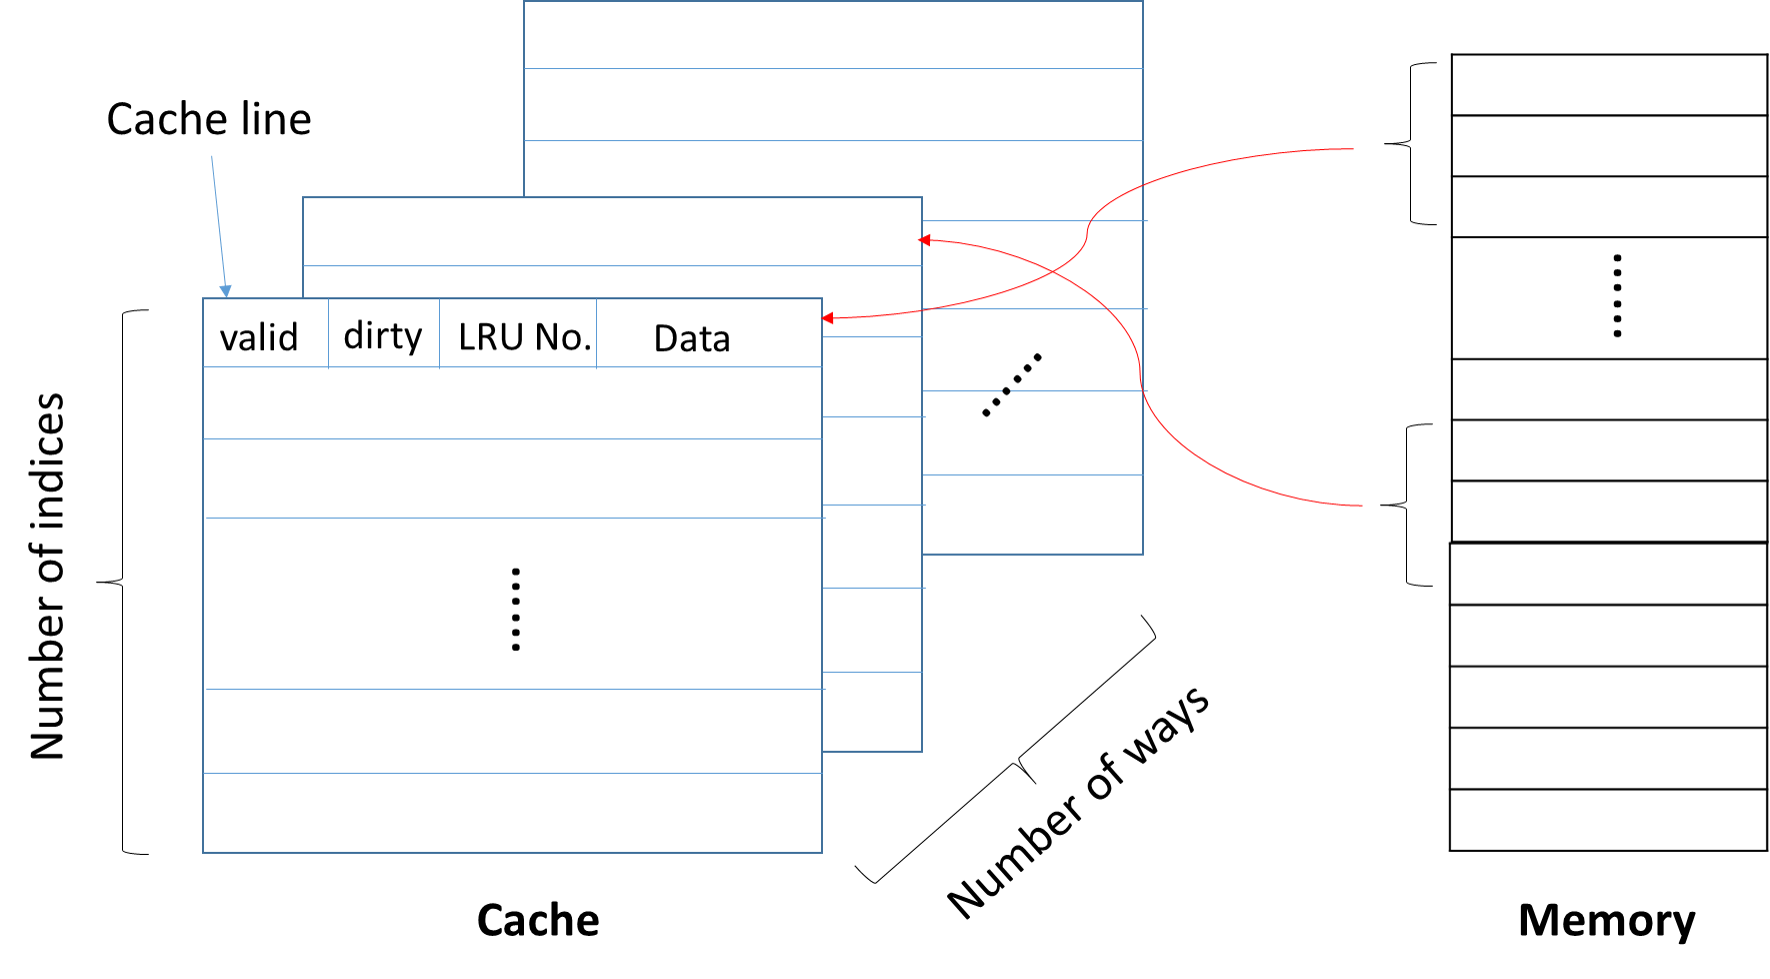
\includegraphics[width = 0.85\linewidth,keepaspectratio]{Cache_and_Memory.png}
\caption{Schematic of memory and cache implementation}
\label{fig:cache_vs_memory}
\end{figure*}

\subsubsection{Memory}
The memory class inherits from the storage class, it implements the methods inherited from the Storage class straightforwardly. The data is saved in an integer array. The pointer to the next level is set to a null pointer. 

\subsubsection{Cache}
We designed and implemented a multiple-way associative cache with write back/through, LRU/Random policies. The cache class also inherits from the Storage class. It consists of multiple cache lines as the basic building stones.
\paragraph{Cache line}
 The cache line is defined using a struct. It has a boolean field called valid that indicates if this cache line is empty or not, a boolean field called dirty that indicates if the content in the cache line is newer than that in the lower level storage. The lru field indicates its priority in the LRU caching mechanism. It also contains a pointer that references an array of 8-bytes integers that served as the data blocks.

The cache consists of a two-dimensional array of cache lines. The rows correspond to indices of memory blocks, the columns correspond to the ways associated to the same index. Number of rows * Number of columns = the total size of cache. The size of the cache, number of ways and number of index can be set at the initialization stage.

\paragraph{Cache functions}
The inCache method takes an address and return the cache line if the address exists in the cache or null pointer if not. Since the memory address starts from 0, it calculates the block index as (address / cache line size) and tag value as (address $\%$ cache line size). The block size corresponds to the index in the cache array. Then it iterates all ways of cache lines attached to that index to see if any tag matches the tag of this address. If there is any match, it returns the position of the cache line otherwise -1. 

The evict method takes a requested address and return an empty cache line corresponding to that address. It looks up in the cache array and search for an empty line of that address, which means that the valid flag is  false. If such a line exists, it returns the line's position. If all lines are occupied, which means all valid flags is to true, it evicts a line according to the eviction policies. We implemented two eviction policies: (1) random eviction (2) LRU eviction. Under the former scenario, a random number between [0, number of ways - 1] is generated. If the dirty tag of this cache line is true, which means it contains newer value than the lower level of storage, it will be written to the lower level of storage. The cache line is emptied and the position of it is returned. The LRU is implemented as follows. Each cache line at a specific index is assigned a LRU number. When a line at this index is updated, its LRU number is set to 0, all others are incremented by 1. Then higher number means the less recent. 

The load method allows us to read a block starting at a specific address in memory. It first checks if the address exists in the current cache by calling the inCache method. If the returned position is -1, there is a cache miss, it will call the the next level of storage, which can be another cache or the memory. The data will be passed along the hierarchical call chain. The newly loaded data have to be written into the cache. The available space is created by calling the evict method. If the returned position is not -1, there is a cache hit. The data in the current cache line is copied and passed up. 

The store method allows us to write an array of data blocks into a specific address in memory. First it checks if the cache line corresponding to that address exists in the cache by calling inCache method. If yes, report a cache hit and copy the data blocks into the current level of cache. Two write policies are implemented:(1) write back (2) write through. In the former scenario, just set the dirty flag of the cache line be true, update the LRU numbers, we are all set. In the latter scenario, we still need to call the store method in the next level of storage. If the address doesn't have a corresponding cache line in the cache, report a cache miss. The load method is called to bring the data blocks at the address into cache. Then it's treated like a cache hit case. 


% multiple-way associative cache with write allocate, LRU 


\subsection{CPU}
\subsection{Pipeline}
\subsection{Assembler and benchmarks}
The assembler takes the instructions in assembly language and encode them into 32-bit integers. The assembler executes in two passes, in the first pass, it strip all the comments that starts with $\#$ symbol and store all labels into a label map, which has the value as the line number. In the second pass, it skips all label-only clause and replace the labels in other clauses with the relative line numbers. It supports type I, II and III instructions. 
All opcodes can be looked up in a preloaded map. 

We implemented the following benchmark programs: (1) Exchange sort (2) Matrix multiplication (3) Matrix multiplication with SIMD.
\begin{algorithm}[]
\SetAlgoLined
 l = length of A\;
 \For{ i from 0 to l - 2}{
	\For{ j from i + 1 to l - 1} {
    	\eIf{A[i] > A[j]}{
        	swap A[i] and A[j]\;
        }{continue;}
    }
 }
 \caption{Exchange sort(integer array A)}
\end{algorithm}

\begin{algorithm}[]
\SetAlgoLined
 a = number of rows in L\;
 b = number of columns in L\;
 c = number of columns in R\;
 Create result matrix res of size a*c, initialized with 0s\;
 \For{ i from 0 to a - 1}{
	\For{ j from 0 to c - 1}{
    	\For{ k from 0 to b - 1}{
        	res[i][j] += L[i][k]*R[k][j]\;
        }
    }
 }
 return res\;
 \caption{Matrix multiplication(left matrix L, right matrix R)}
\end{algorithm}

\begin{algorithm}[]
\SetAlgoLined
 Create result matrix res of size 4, initialized with 0s\;
 Flatten L into a vector v1 of size 8 by rows\;
 Flatten R into a vector v2 of size 8 by columns\;
Create vector v3 with size 8\;
 \For{ i from 0 to 7}{
	v3[i] = v1[i] * v2[i]\;
 }
  \For{ i from 0 to 3}{
	\For{ j from 0 to 3}{    	
        	res[i][j] = v3[(i*2+j)*2] + v3[(i*2+j) + 1]\;
    }
 }
 return res\;
 \caption{2 by 2 Matrix multiplication with SIMD(left matrix L, right matrix R)}
\end{algorithm}

\subsection{User interface}
\section{Performance evaluation}
\section{Summary}



\end{document}